\chapter{Personnaliser votre compte}\label{chap:personnaliserCompte}
\begin{figure}
    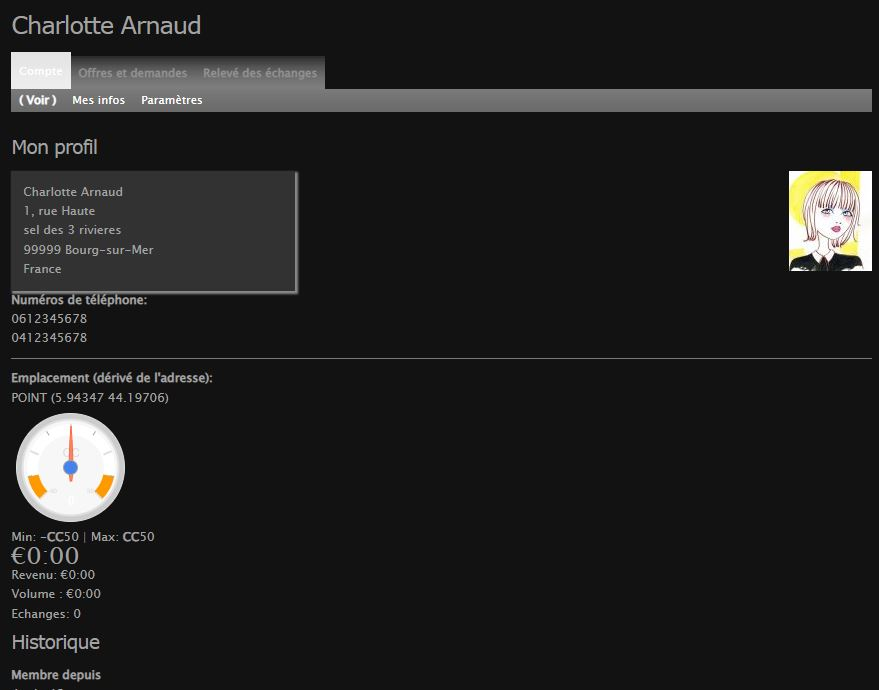
\includegraphics[width=\linewidth]{144-mon_compte_voir}
    \caption[Page de profil]{Page de profil (sous-onglet <<~Voir~>> de l'onglet <<~Compte~>>)}
    \label{fig:monCompteVoir}
\end{figure}

{\slshape
\noindent Dans ce chapitre, nous verrons comment mettre à jour les éléments de votre profil, compléter vos informations, modifier (quelque peu) l'affichage des pages, rédiger un petit texte de présentation, etc.; la plupart des membres négligent tout cela et c'est bien dommage pour les autres.}

\section[Onglet «~Mon Compte~»]{Onglet «~Mon Compte~» du menu utilisateur}\label{page:compte_offres_demandes}

Dans le menu utilisateur (voir \vref{sec:menuUtilisateur}), cliquez sur \liensmenu{Mon compte} pour accéder à votre \index{fiche de profil}page de profil (Fig. \vref{fig:monCompteVoir}). Celle-ci comporte un menu contextuel\index{menu contextuel!de l'onglet Mon Compte du menu utilisateur} avec trois liens:

\begin{description}
    \item[\liensmenu{Compte}] Le premier lien est celui où s'effectue la personnalisation de votre compte; c'est lui qui fait l'objet de ce chapitre.
    \item[\liensmenu{Offres et Demandes}] Le deuxième lien affiche la liste des offres et des demandes que vous avez publiées --- et que vous n’avez pas encore effacées ---, nous verrons l'utilité de ce lien plus loin, notamment à la section <<~Durée de validité de l'annonce~>> (p. \pageref{sec:dureeValiditeAnnonce}, voir aussi Fig. \ref{fig:compte_offres_demandes}, p. \pageref{fig:compte_offres_demandes}).
    \item[\liensmenu{Relevé des échanges}] Le troisième lien n’est pas utilisé au \CdS. 
\end{description}

\subsec{Sous-onglets de l’onglet «~Compte~» }

Le premier lien \liensmenu{Compte}
%%%
\footnote{La distinction entre les liens \liensmenu{Mon compte} et \liensmenu{Compte} introduit un peu de confusion: \liensmenu{Mon compte} est un lien du menu permanent utilisateur (Fig. \ref{fig:menuUtilisateur}, p. \pageref{fig:menuUtilisateur}), ce lien amène au menu contextuel de la figure \vref{fig:monCompteVoir}; \liensmenu{Compte} est le premier lien de ce menu et il comprend les trois sous-onglets qui font l'objet de cette section.}
%%%
comporte un sous-menu avec trois liens \liensmenu{Voir}, \liensmenu{Mes infos} et \liensmenu{Paramètres}. Lorsque vous cliquez sur le lien \liensmenu{Mon compte} du menu utilisateur, vous arrivez sur le sous-onglet \liensmenu{Voir} (Fig. \ref{fig:monCompteVoir}%
%%%
\footnote{Aux figures \vrefrange{fig:monCompteVoir}{fig:pageParametres}, le sous-onglet ouvert est indiqué entre parenthèses.})
%%%
où se trouvent vos informations de \index{fiche de profil}profil: prénom, nom, adresse, téléphone(s) ainsi qu'une photo si vous l'avez ajoutée --- voir <<~Ajouter une photo de profil~>>, \vpageref{sec:insererImage}.

Tout ce qui figure au-dessous du trait horizontal n’est pas utilisé au \CdS
%%%
\footnote{Attention, les coordonnées gps, \noncliquables{Emplacement (dérivé de l'adresse)}, ne sont pas très fiables, ne les utilisez pas pour vous rendre chez l'adhérent ou l'adhérente.}.
%%%

La personnalisation proprement dite s’effectue dans les deux onglets suivants.

\index{Profil!mise à jour|(}
\section{Sous-onglet «~Mes infos~»}
\label{page:completerInfosPerso}

Les champs \noncliquables{Pays}, \noncliquables{Prénom} et \noncliquables{Localité}\index{Localite@Localité}, repérés par une astérisque rouge (Fig. \ref{fig:mesInfos}, p. \pageref{fig:mesInfos}), sont les champs indispensables pour la création du compte, n’y touchez pas.

\rem{La localité\index{Localite@Localité} n'est pas celle de votre adresse postale --- celle-ci figure au-dessous, dans le champ \noncliquables{Ville} --- mais la désignation de votre \sel. Aujourd'hui, avec la mise en sommeil des \sel{} de Sisteron et de Laragne, seul subsiste le \CdS{}
%%%
\footnote{Sauf pour Charlotte \textsc{Arnaud}, et Zoé Test que nous rencontrerons au chapitre \ref{chap:fonctionnalitesCompte}, toujours adhérentes du \sel{} des 3 Rivières à Sisteron ! Nous verrrons plus loin l'intérêt de la chose.}.}
%%%

Normalement, les autres champs ont été remplis à la création de votre compte par un \index{administrateur local}administrateur local, sauf peut-être un second numéro de téléphone que vous pouvez ajouter et, bien sûr, le champ optionnel \noncliquables{Je me présente}. Si certaines informations sont absentes, il vous faut les ajouter
%%%
\footnote{ou demander à un \index{administrateur local}administrateur local de le faire pour vous.}. 
%%%
À la figure \ref{fig:mesInfos}, le profil de Charlotte est vide à l'exception des trois champs indispensables pour la création du compte. En appendice (p. \pageref{fig:profilCharlotteComplet}), vous trouverez l'ensemble des champs du profil de Charlotte correctement remplis --- lorsque les champs sont correctement remplis, la page de profil est celle de la figure \vref{fig:monCompteVoir}.

Le champ \noncliquables{Je me présente} est optionnel. C'est cependant une bonne idée de le compléter surtout pour les membres moins connus comme les nouveaux membres --- mais pas seulement; c'est un élément de convivialité important.

Notez que les informations données ici ne sont visibles que par les membres de notre \sel, c’est la garantie apportée par le RGPD\index{RGPD|(} (Règlement Général sur la Protection des Données).
\begin{figure}
    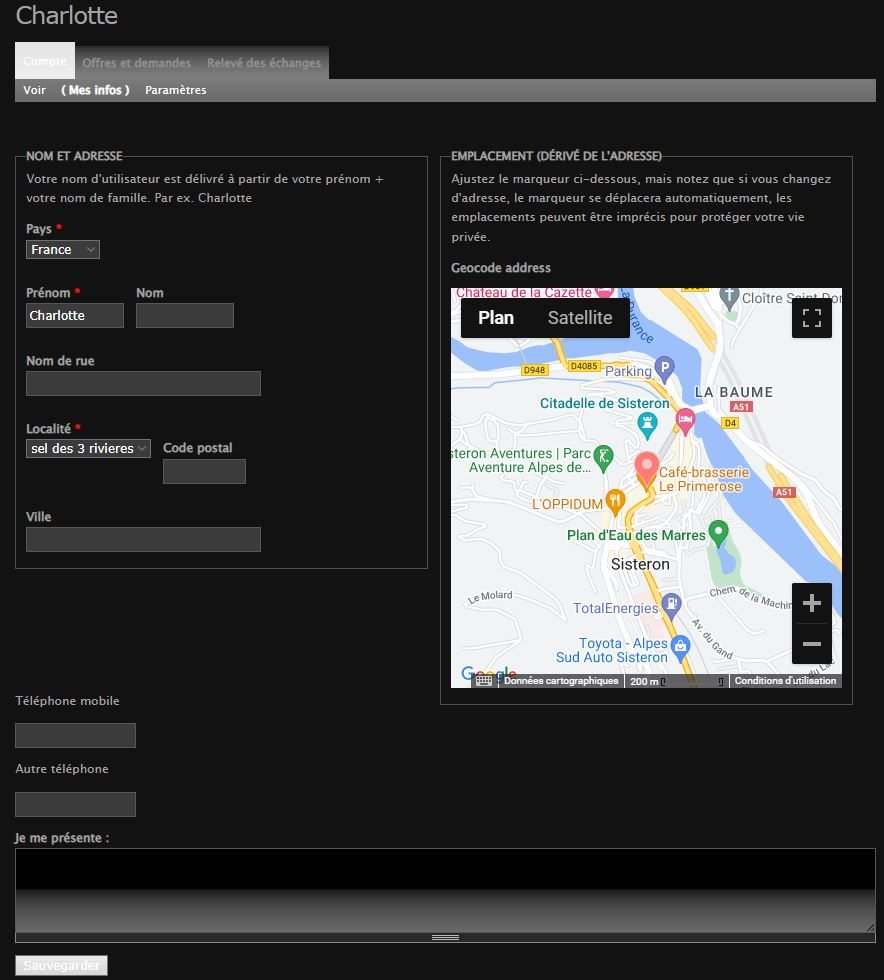
\includegraphics[width=\linewidth]{150-mon_compte_mes_infos}
    \caption[Onglet <<~Mes infos~>>]{Onglet <<~Mes infos~>> (sous-onglet de l'onglet <<~Compte~>>)}
    \label{fig:mesInfos}
\end{figure}
\begin{mybox}[colbacktitle=MidnightBlue]{À propos du RGPD}
    Le RGPD a pour but premier --- mais pas unique, voir la dernière partie de cet encadré --- de protéger les \index{donnees personnelles@données personnelles}données personnelles de chacun de nous. Dans le cadre du \sel{}, il s'agit essentiellement de nos numéros de téléphone et de notre adresse postale. Le site de \CF{} répond à ce besoin en ce sens que les données qui apparaissent dans la \index{fiche de profil}fiche de profil ne peuvent pas être vues par des extérieurs, \cad{} des gens qui ne sont pas membres du \CdS.
    \aster
    Le RGPD stipule également qu'on ne peut pas demander des informations personnelles au delà de celles strictement nécessaires au fonctionnement de (dans notre cas) l'association du \sel{} --- \ex, toujours dans notre cas, la date de naissance ou la nationalité ne sont pas utiles pour le fonctionnement du \sel{} elles ne doivent pas être demandées. Certains \sel{} demandent la date de naissance pour fêter les anniversaires alors  qu'ils ne devraient demander que le jour et le mois de naissance, les seules informations nécessaires pour cela.
    
    Par contre, pour réaliser des échanges, ce qui est le but inscrit dans les statuts ou dans le règlement intérieur de l'association \CdS, il est nécessaire de pouvoir contacter les autres membres, il est donc légitime de demander adresse postale et numéro de téléphone.
    \aster
    Mais le RGPD comporte aussi des obligations, notamment l'obligation de réciprocité qui signifie qu'un membre du \sel{} ne peut pas avoir accès aux informations des autres membres tout en cachant les siennes. 
    
    La conséquence de cette obligation de réciprocité est que tous les membres doivent fournir les mêmes informations les concernant, \cad{} leur nom, leur adresse postale et (au moins) un numéro de téléphone --- sauf bien sûr pour un membre qui n'aurait pas de téléphone, s'il en existe !
\end{mybox}\index{RGPD|)}

\medskip

Enfin, en fonction de l'adresse indiquée, la carte située à droite sera mise à jour de façon plus ou moins précise. Lorsqu'aucune adresse n'est fournie, l'emplacement par défaut semble être à Sisteron%
%%%
\footnote{Peut-être parce que lorsque j'ai demandé l'ouverture du site \CF{} pour les 3 \sel{}, j'étais moi-même adhérent du \sel{} de Sisteron !} 
%%%
(Fig. \ref{fig:mesInfos}).

Si vous avez ajouté ou modifié certaines informations, \textbf{n'oubliez pas d'aller tout en bas de la page et de cliquer sur le bouton} \autresliens{Sauvegarder}.
\index{Profil!mise à jour|)}

\section{Sous-onglet «~Paramètres~»}
\begin{figure}
    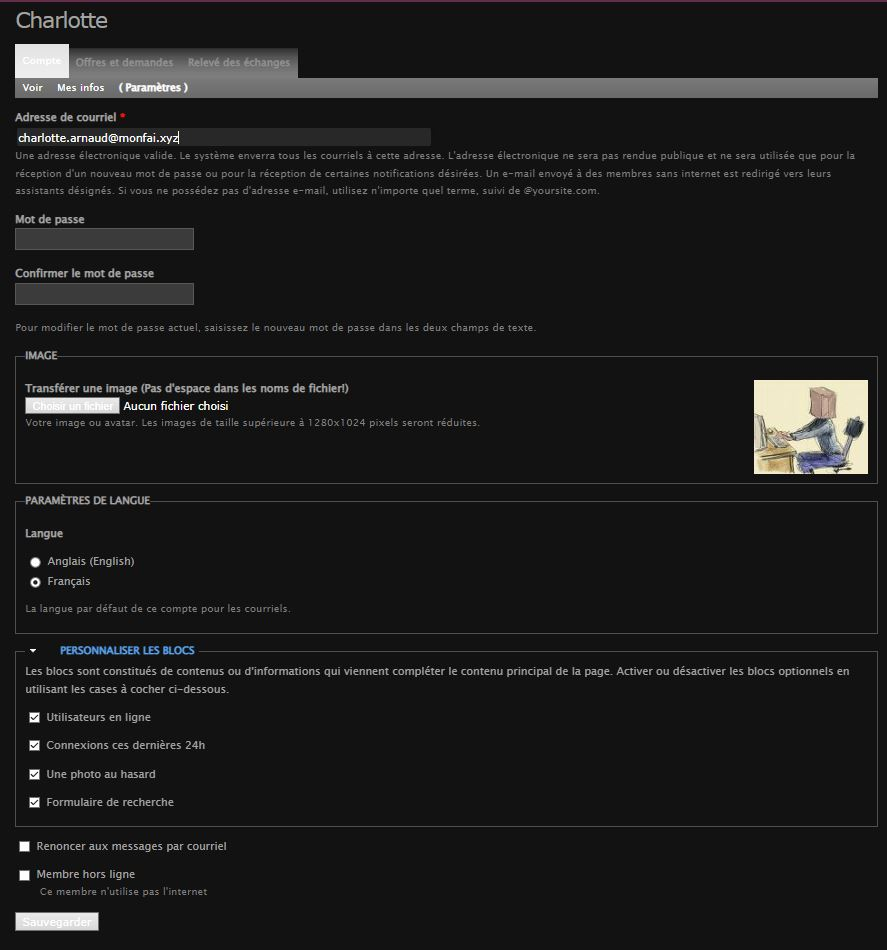
\includegraphics[width=\linewidth]{160-mon_compte_parametres}
    \caption[Onglet <<~Paramètres~>>]{Onglet <<~Paramètres~>> (sous-onglet de l'onglet <<~Compte~>>)}
    \label{fig:pageParametres}
\end{figure}

Cette page est représentée à la figure \ref{fig:pageParametres}, \vpageref{fig:pageParametres}.

\subsec{Adresse de courriel}\index{adresse de courriel!la changer}

Ce champ est marqué d'une astérisque rouge car cette adresse est indispensable pour l'existence du compte%
%%%
\footnote{Sauf pour les membres dits \og Membres hors ligne\fg, voir \vpageref{sec:membresHorsLigne}.}.
%%%
Celui-ci a été créé avec l'adresse que vous avez fournie lors de votre adhésion (voir Chapitre I, notamment la section <<~Activation du compte~>>). Par la suite, vous pouvez la changer ici si vous le souhaitez.

La nouvelle adresse doit être une adresse électronique valide: \textbf{attention aux fautes de frappe}, relisez-vous soigneusement.

\subsec{Changer le mot de passe}\index{mot de passe!réinitialiser}\label{sec:changerMotDePasse}

Si vous devez changer votre mot de passe, notamment dans le cas où celui-ci a été compromis%
%%%
\footnote{Contrairement à ce qu'on lit parfois, il n'est pas nécessaire de changer de mot de passe tant qu'il n'y a aucune raison de penser qu'il a été compromis.},
%%%
 c’est ici que vous pouvez le faire: entrez votre nouveau mot de passe, confirmez-le puis allez en fin de page pour cliquer sur \autresliens{Sauvegarder}.

\subsec{Renoncer aux messages par courriel}

C’est également sur cette page que vous pouvez renoncer aux messages du \CdS{} (avant dernière case à cocher en bas de la page). Cela signifie que vous ne recevrez plus les messages diffusés par le \sel{} (offres, demandes, actualités, etc.), il faudra alors vous connecter régulièrement sur le site pour connaître son activité.En général, les adhérent(e)s préfèrent recevoir les informations dans leur boîte mél et ne cochent pas cette case. 

Si vous la cochez, n'oubliez de cliquer sur \autresliens{Sauvegarder} en bas de la page%
%%%
\footnote{Sans entrer dans les détails, disons qu'il existe quelques rares cas où une information est diffusée par courriel sans figurer sur le site. Donc, sauf à avoir une raison impérieuse pour cela, ne cochez pas cette case!}.
%%%

\subsec{Membres hors-ligne}\label{sec:membresHorsLigne}
\index{Membres!hors ligne}

La dernière case à cocher en bas de la page, intitulée \noncliquables{Membre hors ligne}, ne devrait pas vous concerner puisque vous êtes sur le site; un membre hors ligne est un membre qui n'a pas de connexion internet.

\subsec{Ajouter une photo de profil}\label{sec:insererImage}
\index{photo!de profil}\index{image!transférer}

Dans le cadre \noncliquables{IMAGE}, vous avez la possibilité d’inclure une image à télécharger depuis votre terminal (ordinateur, tablette, smartphone, etc.). Pour cela:
\begin{enumerate}
    \item cliquez sur \autresliens{Choisir un fichier};
    \item une fenêtre s’ouvre sur votre terminal;
    \item naviguez jusqu’au fichier image (format \termecode{jpeg} ou \termecode{png}) à transférer et ouvrez-le;
    \item son nom apparaît à la place du texte \noncliquables{Aucun fichier choisi};
    \item allez en bas de la page et cliquez sur \autresliens{Sauvegarder}.
\end{enumerate}
Notez que les étapes 2 et 3 dépendent de votre système d’exploitation, Windows ou IOS ou Linux (ou plutôt Linuces).

\subsec{Paramètres de langue}

Le cadre \noncliquables{PARAMÈTRES DE LANGUE} est sans objet, le site n’existant qu’en français.

\subsec{Supprimer l'affichage de certains blocs}\label{sec:supprimerBlocs}
\index{bloc!supprimer|(}

Enfin, le cadre \noncliquables{PERSONNALISER LES BLOCS} permet de supprimer certains blocs normalement présents sur la plupart des pages mais qui ne vous intéressent peut-être pas. Ce sont les blocs suivants (voir Fig. \ref{fig:vueGeneralePage}, p. \pageref{fig:vueGeneralePage}) :
\begin{itemize}
    \item colonne de gauche, \index{bloc!Utilisateurs en ligne}\noncliquables{Utilisateurs en ligne}: les membres connectés en même temps que vous;
    \item au-dessous, \index{bloc!Connexions ces dernières 24h} \noncliquables{Connexions ces dernières 24h}: les membres qui se sont connectés durant les dernières 24h;
    \item en bas colonne de gauche, \index{bloc!Une photo au hasard}\noncliquables{Une photo au hasard}: affiche une photo choisie au hasard dans un des albums du site;
    \item en haut à droite, \index{bloc!de recherche}le bloc de recherche: permet de faire une recherche sur le site.
\end{itemize}

Pour que ces blocs n’apparaissent plus sur vos pages,  décochez la case correspondante puis cliquez sur \autresliens{Sauvegarder} en bas de la page.\index{bloc!supprimer|)}
